\documentclass[border=5pt]{standalone}
\usepackage{tikz}
\usetikzlibrary{positioning, fit, decorations.pathreplacing}
\usepackage{mathtools}

\begin{document}
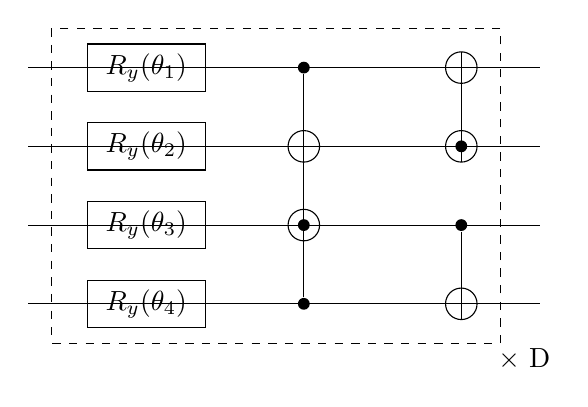
\begin{tikzpicture}[
    gate/.style={draw, minimum width=1.5cm, minimum height=0.6cm},
    control/.style={circle, fill, minimum size=0.15cm, inner sep=0pt},
    target/.style={circle, draw, minimum size=0.4cm, inner sep=0pt, path picture={
        \draw (path picture bounding box.north) -- (path picture bounding box.south);
        \draw (path picture bounding box.east) -- (path picture bounding box.west);
    }},
]

% 量子比特线
\foreach \y in {0, 1, 2, 3} {
    \draw (-0.5, -\y) -- (6, -\y);
}

% 旋转门
\node[gate] (g1) at (1, 0) {$R_y(\theta_1)$};
\node[gate] (g2) at (1, -1) {$R_y(\theta_2)$};
\node[gate] (g3) at (1, -2) {$R_y(\theta_3)$};
\node[gate] (g4) at (1, -3) {$R_y(\theta_4)$};

% CNOT门
\node[control] (c1) at (3, 0) {};
\node[target] (t1) at (5, -1) {};
\draw (c1) -- (c1 |- t1) -- (t1);

\node[target] (t2) at (3, -1) {};
\node[control] (c2) at (3, -2) {};
\draw (c2) -- (c2 |- t2) -- (t2);

\node[target] (t3) at (3, -2) {};
\node[control] (c3) at (3, -3) {};
\draw (c3) -- (c3 |- t3) -- (t3);

\node[target] (t4) at (5, -3) {};
\node[control] (c4) at (5, -2) {};
\draw (c4) -- (c4 |- t4) -- (t4);

\node[target] (t5) at (5, 0) {};
\node[control] (c5) at (5, -1) {};
\draw (c5) -- (c5 |- t5) -- (t5);

% 虚线框
\draw[dashed] (-0.2, 0.5) rectangle (5.5, -3.5);

% 重复标记
\node at (5.8, -3.7) {$\times$ D};

\end{tikzpicture}
\end{document}